% !TEX root = ../../prj4projektdokumentation.tex
% SKAL STÅ I TOPPEN AF ALLE FILER FOR AT MASTER-filen KOMPILERES 

\section{Ikke funktionelle krav}

\subsection{Spændingsregulator}
\begin{enumerate}
	\item Maks belastning af spændingsregulatoren er 20VA
	\item Nominel spænding på primær siden er 24VAC
	\item Nominel spænding på sekundær siden er 4VAC
	\item Maks strøm er 5A	
\end{enumerate}

\subsection{Måleenhed}

\begin{enumerate}
	\item Måle spændingen ved trinskifteren og forbrugerne mellem 0 og 8 V, $\pm$ 200mV 
	\item Måle strømniveauet ved trinskifteren og forbrugerne mellem 0 og 5A, $\pm$ 100mA
	\item Måle power factor $\pm$ 10$\%$
\end{enumerate}

\subsection{Brugergrænseflade}

\begin{enumerate}
	\item Automatisk mode
	\begin{figure}[htbp] % (alternativt [H])
		\centering
		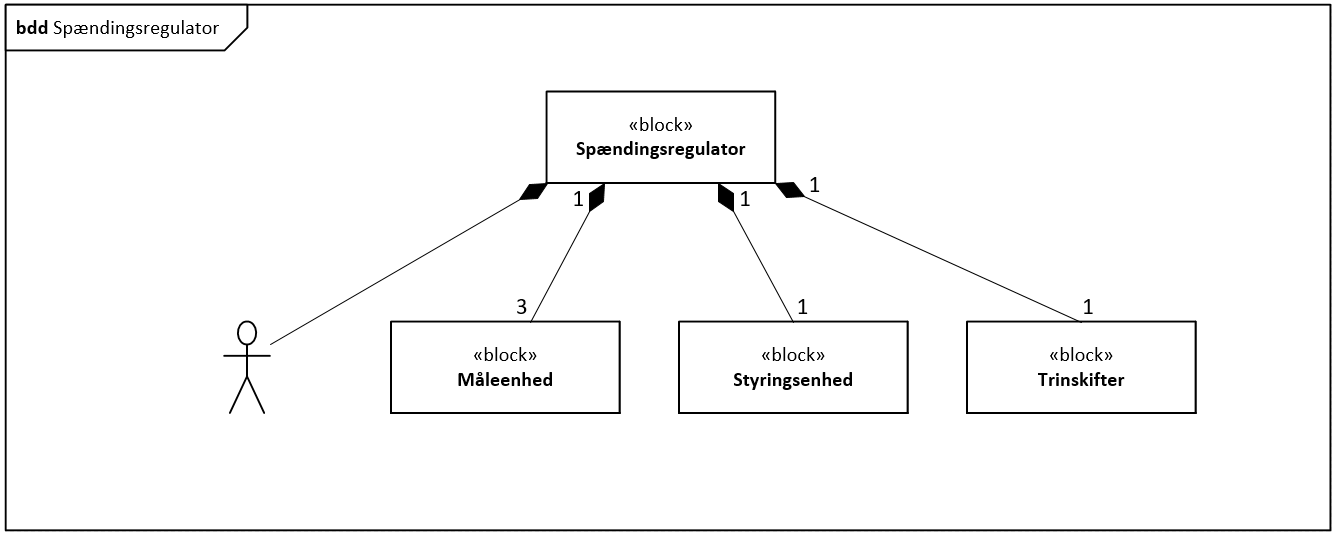
\includegraphics[width=0.9\textwidth]{Figure/BDDSpaendingsregulator}
		\caption{HMI Automatisk mode}
		\label{fig:HMIAutomatikMode}
	\end{figure}

	\item Manuel mode
	\begin{figure}[htbp] % (alternativt [H])
	\centering
	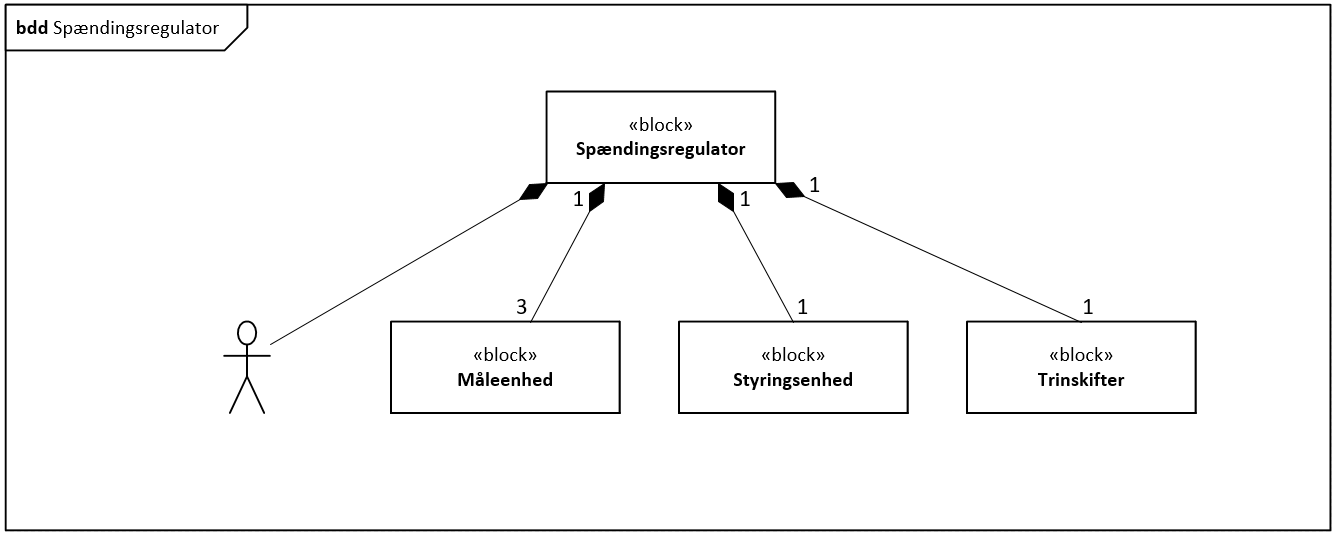
\includegraphics[width=0.9\textwidth]{Figure/BDDSpaendingsregulator}
	\caption{HMI Manuel mode}
	\label{fig:HMIManuelMode}
	\end{figure}
\end{enumerate}



